\chapter{Threads}
Threads in a process share data (global variable) and code. Each thread has its own stack for function calls. Each thread can allocate its own \emph{Thread Local Storage} (TLS), which represents a way to share data which are private to the thread.

\begin{figure}[hbtp]
\centering
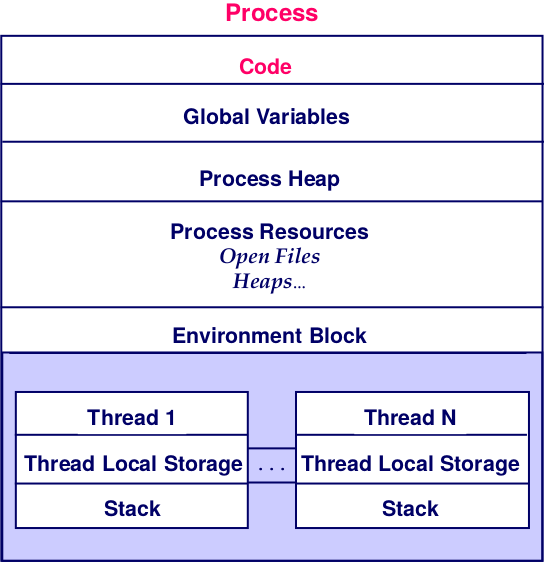
\includegraphics[scale=0.35]{images/windows_threads/process_threads.png}
\caption{Processes and threads}
\end{figure}

Threads are scheduled and run independently. Windows works with threads as atomic unit of execution and scheduling.
\\
Benefits:
\begin{itemize}
\item Simpler program models;
\item Faster code, in many cases, when it is possible to exploit multiple processors or inherent application parallelism, i.e.,\@ concurrency can catch real concurrency;
\item Reliable, understandable, maintainable code.
\end{itemize}
Risks:
\begin{itemize}
\item Difficult to debug;
\item Slower performance, in some cases;
\item Potential defects.
\end{itemize}

\section{Creating a thread}
Thread creation needs to specify the thread's start address within the process' code, the stack size and the stack consume space within the process' address space, 

\begin{verbatim}
HANDLE CreateThread (
  LPSECURITY_ATTRIBUTES lpsa,
  DWORD cbStack,
  LPTHREAD_START_ROUTINE lpStartAddr,
  LPVOID lpvThreadParm,
  DWORD dwCreate,
  LPDWORD lpIDThread
);
\end{verbatim}

\paragraph{Returned value}
\begin{itemize}
\item A thread's identifier value and its handle;
\item A \texttt{NULL} handle value indicates failure.
\end{itemize}

\paragraph{Parameters}
\begin{description}
\item [\texttt{lpsa}] Usually \texttt{NULL}. It points to a \texttt{SECURITY\_ATTRIBUTES} structure.
\item [\texttt{cbStack}] Byte size for the new thread's stack. Use \texttt{0} to default to the primary thread's stack size (1~MB).
\item [\texttt{lpStartAddr}] Pointer to the function to be executed. Actually it is the function name, which accepts a single pointer argument and returns a 32-bit \texttt{DWORD} exit code. The thread can interpret the argument as a \texttt{DWORD} or a pointer.
\item [\texttt{lpvThreadParm}] Pointer passed as the thread argument.
\item [\texttt{dwCreate}] If \texttt{0}, the thread is immediately ready to run; if \texttt{CREATE\_SUSPENDED}, the new thread will be in suspended state, requiring a \texttt{ResumeThread} function call to move the thread to the ready state.
\item [\texttt{lpIDThread}] Pointer to a \texttt{DWORD} that receives the new thread's identifier; \texttt{NULL} is ok on W2000/NT.
\end{description}

\subsection{The thread function}
\begin{verbatim}
DWORD WINAPI MyThreadFunction (PVOID pThreadParam) {
  ExitThread (ExitCode);
  /* return ExitCode; */
}
\end{verbatim}

\section{Thread termination}
Threads are terminated by \texttt{ExitProcess}:
\begin{itemize}
\item The process and all its threads terminate;
\item The exit code returned by the thread start function is the same as the process exit code;
\end{itemize}

\begin{verbatim}
VOID ExitThread (DWORD dwExitCode);
\end{verbatim}
A thread can simply return with its exit code. \texttt{ExitThread} is preferred technique and the thread's stack is deallocated on termination. When the last thread in a process terminates, so does the process itself.

\paragraph{Parameter}
\begin{description}
\item [\texttt{dwExitCode}] Exit code for the thread.
\end{description}

It is possible to terminate a thread with \texttt{TerminateThread} but it is dangerous because the thread's stack and other resources will not be deallocated, leading to possible leaks. In fact, it is better to let the thread terminate itself.

A thread will remain in the system until the last handle to it is closed, using \texttt{CloseHandle}\footnote{Similar to UNIX zombies.}, then the thread will be deleted.

\subsection{Thread exit codes}
Any other thread can retrieve the exit code.
\begin{verbatim}
BOOL GetExitCodeThread (
  HANDLE hThread,
  LPDWORD lpdwExitCode
);
\end{verbatim}

\paragraph{Returned value}
\begin{itemize}
\item \texttt{TRUE} if the function succeeds, i.e.,\@ if it is possible to retrieve the exit code;
\item \texttt{FALSE} otherwise.
\end{itemize}

\paragraph{Parameter}
\begin{description}
\item [\texttt{hThread}] Handle to the thread.
\item [\texttt{lpdwExitCode}] Thread's exit code. It could be \texttt{STILL\_ACTIVE} if the thread is running.
\end{description}

\section{Thread identities}
A thread has a permanent \texttt{ThreadId} and it is usually accessed by \texttt{HANDLE}. An \texttt{ID} can be converted to a \texttt{HANDLE}.

\begin{verbatim}
HANDLE GetCurrentThread (VOID);
DWORD GetCurrentThreadId (VOID);
HANDLE OpenThread (
  DWORD dwDesiredAccess,
  BOOL InheritableHandle,
  DWORD ThreadId
);
\end{verbatim}

\paragraph{Returned value}
\begin{itemize}
\item An open \texttt{HANDLE} to the specified thread if the function succeeds;
\item \texttt{NULL} if it fails.
\end{itemize}

\paragraph{Parameter}
\begin{description}
\item [\texttt{dwDesiredAccess}] Access to the thread object.
\item [\texttt{InheritableHandle}] If \texttt{TRUE}, processes created by this process will inherit the handle. Otherwise, the processes do not inherit this handle.
\item [\texttt{ThreadId}] Identifier of the thread to be opened.
\end{description}

\section{Suspend \& resume threads}
Every thread has a \emph{suspend count} and it can execute only if this count is zero. A thread can be create in the \emph{suspended state} and increment or decrement the suspend count of another.

These functions are useful in preventing ``race conditions'', because they do not allow threads to start until initialization is complete but they are unsafe for general synchronization.

\begin{verbatim}
DWORD ResumeThread (HANDLE hThread);
DWORD SuspendThread (HANDLE hThread);
\end{verbatim}

\paragraph{Returned value}
\begin{itemize}
\item The previous suspend count if the function succeeds;
\item \texttt{0xFFFFFFFF} if it fails.
\end{itemize}

\paragraph{Parameter}
\begin{description}
\item [\texttt{hThread}] Handle to the thread to be restarted or suspended.
\end{description}

\section{Waiting for thread termination}
There is no specific function to wait for thread termination. In fact, wait for a thread to terminate is done using general purpose wait functions, which wait for the thread handle to become signaled.
\begin{itemize}
\item \texttt{ExitThread} and \texttt{TerminateThread} set the object to the signaled state, releasing all other threads waiting on the object;
\item \texttt{ExitProcess} sets the process' state and all it threads' states to signaled.
\end{itemize}

\begin{verbatim}
DWORD WaitForSingleObject (
  HANDLE hObject,
  DWORD dwTimeOut
);
\end{verbatim}

\paragraph{Parameters}
\begin{description}
\item [\texttt{hHandle}] Handle to the object.
\item [\texttt{dwTimeOut}] Timeout interval in milliseconds.
\begin{description}
\item [\texttt{0}] Function returns immediately after testing the state of the specified object;
\item [\texttt{INFINITE}] No timeout. Wait forever for a thread to terminate.
\end{description}
\end{description}

\begin{verbatim}
DWORD WaitForMultipleObjects (
  DWORD cObjects,
  LPHANDLE lphObjects,
  BOOL fWaitAll,
  DWORD dwTimeOut
);
\end{verbatim}

\paragraph{Parameters}
\begin{description}
\item [\texttt{cObjects}] Number of handles in the array pointed to by \texttt{lphObjects}. It cannot exceed \texttt{MAXIMUM\_WAIT\_OBJECTS}, i.e.,\@ 64.
\item [\texttt{lphObjects}] Array of object handles.
\item [\texttt{fWaitAll}]
\begin{description}
\item [\texttt{TRUE}] indicates to wait for all the threads to terminate.
\end{description}
\item [\texttt{dwTimeOut}] Timeout interval in milliseconds.
\begin{description}
\item [\texttt{0}] Functions returns immediately after testing the state of the specified object;
\item [\texttt{INFINITE}] No timeout. Wait forever for a thread to terminate.
\end{description}
\end{description}

\paragraph{Returned value}
\begin{itemize}
\item \texttt{WAIT\_OBJECT\_0}: The thread terminated, if calling \texttt{WaitForSingleObject} or \texttt{WaitForMultipleObject} with \texttt{fWaitAll} set;
\item \texttt{WAIT\_OBJECT\_0 + n}, where \texttt{0 <= n < cObjects}: Subtract \texttt{WAIT\_OBJECT} from the returned value to determine which thread terminated when calling \texttt{WaitForMultipleObject} with \texttt{fWaitAll} unset;
\item \texttt{WAIT\_TIMEOUT}: Timeout period elapsed;
\item \texttt{WAIT\_ABANDONED} Not possible with thread handles;
\item \texttt{WAIT\_FAILED}: Call \texttt{GetLastError} for thread-specific error code.
\end{itemize}

\section{The C library and threads}
Nearly all programs and thread functions use the C library, which is normally not ``thread safe'' because it uses global variables for the process, i.e.,\@ for all threads and not for the single thread. The C function \texttt{\_beginthreadex} has exactly the same parameters as \texttt{CreateThread}.

Cast \texttt{\_beginthreadex} return value to \texttt{(HANDLE)} and use \texttt{\_endthreadex} in place of \texttt{ExitThread}, included in \texttt{process.h}.

\section{Synchronization objects}
A thread can wait for another to terminate (using \texttt{ExitThread}) by waiting on the thread handle using \texttt{WaitForSingleObject} or \texttt{WaitForMultipleObjects}. A process can wait for another process to terminate (using \texttt{ExitProcess}) in the same way. Other common methods are reading from a pipe or socket that allows one process or thread to wait for another to write to the pipe or socket. File locks are specially for synchronizing file access.

Windows provides four other objects specifically designed for thread and process synchronization. Three are kernel objects (they have \texttt{HANDLE}s):
\begin{itemize}
\item Events, i.e.,\@ specific synchronization primitive for Windows. There is no equivalence in UNIX systems;
\item Semaphores;
\item Mutexes.
\end{itemize}
Critical section is the fourth object type which can only synchronize threads within a process. Often it is the most efficient choice because it is not a kernel object and it is applicable to many scenarios. Only one thread at a time can be in a specific critical section. There is a \texttt{CRITICAL\_SECTION} type.

\subsection{\texttt{CRITICAL\_SECTION}s}
\begin{verbatim}
VOID InitializeCriticalSection (
  LPCRITICAL_SECTION lpcsCriticalSection);
VOID DeleteCriticalSection (
  LPCRITICAL_SECTION lpcsCriticalSection);
VOID EnterCriticalSection (
  LPCRITICAL_SECTION lpcsCriticalSection);
VOID LeaveCriticalSection (
  LPCRITICAL_SECTION lpcsCriticalSection);
VOID TryCriticalSection (
  LPCRITICAL_SECTION lpcsCriticalSection);
\end{verbatim}

\begin{itemize}
\item \texttt{EnterCriticalSection} blocks a thread if another thread is in the section;
\item \texttt{TryCriticalSection} simply tests if the critical section is busy, avoiding blocking;
\item \texttt{LeaveCriticalSection} unblocks waiting thread when the ``owning'' one executes it.
\end{itemize}
Common usage is to allow threads to access global variable, which should be declared \texttt{volatile}.

\texttt{CRITICAL\_SECTION}s test in user-space, therefore they are faster because there is no kernel call. Usually they are faster than mutexes but not always because performance is affected by different factors, e.g.,\@ number of threads, number of processes and amount of thread contention.

\subsection{Mutuxes}
\emph{Mutexes} can be named and have \texttt{HANDLE}s, i.e.,\@ they are kernel objects. They can be used for interprocess synchronization and they are owned by a thread rather than a process.

Threads gain mutex ownership by waiting on mutex handle with standard \texttt{WaitForSingleObject} or \texttt{WaitForMultipleObjects}. Threads release ownership with \texttt{ReleaseMutex}.

A thread can acquire a specific mutex several times but must release the mutex the same number of times, e.g.,\@ with nested transactions. A mutex becomes ``abandoned'' if its owning thread terminates.

\begin{verbatim}
HANDLE CreateMutex (
  LPSECURITY_ATTRIBUTES lpsa,
  BOOL fInitialOwner,
  LPCTSTR lpszMutexName
);
\end{verbatim}

\paragraph{Returned value}
\begin{itemize}
\item An open \texttt{HANDLE} to the newly created mutex object, if the function succeeds;
\item \texttt{NULL}, if it fails.
\end{itemize}

\paragraph{Parameters}
\begin{description}
\item [\texttt{lpsa}] Usually \texttt{NULL}. It points to a \texttt{SECURITY\_ATTRIBUTES} structure.
\item [\texttt{fInitialOwner}] If \texttt{TRUE}, it gives the calling thread immediate ownership of the new mutex.
\item [\texttt{lpszMutexName}] Pointer to a \texttt{NULL}-terminated pathname. Mutexes are unnamed if it is \texttt{NULL}.
\end{description}

\begin{verbatim}
BOOL ReleaseMutex (
  HANDLE hMutex
);
\end{verbatim}

It frees a mutex that the calling thread owns and it fails if the thread does not own it. If a mutex is abandoned, a wait will return \texttt{WAIT\_ABANDONED\_0}.

\paragraph{Mutex naming}
Naming a mutex permits to use it in more than one process. It is not necessary to name a mutex used in a single process. Named mutex can be opened using \texttt{OpenMutex}.

\subsection{Events}
\emph{Events} can release multiple threads from a wait simultaneously when a single event in signaled, with either \texttt{PulseEvent} or \texttt{SetEvent}.

\begin{itemize}
\item A \emph{manual-reset} event can signal several threads simultaneously and must be reset by the thread;
\item A \emph{auto-reset} event signals a single thread, and the event is automatically reset.
\end{itemize}

\begin{verbatim}
HANDLE CreateEvent (
  LPSECURITY_ATTRIBUTES lspa,
  BOOL fManualReset,
  BOOL fInitialState,
  LPTCSTR lpszEventName
);
\end{verbatim}

\paragraph{Returned value}
\begin{itemize}
\item An \texttt{HANDLE} to the created event object if the function succeeds;
\item \texttt{NULL} if it fails.
\end{itemize}

\paragraph{Parameters}
\begin{description}
\item [\texttt{lpsa}] Usually \texttt{NULL}. It points to a \texttt{SECURITY\_ATTRIBUTES} structure.
\item [\texttt{fManualReset}] If \texttt{TRUE}, the function creates a manual-reset event object; if \texttt{FALSE}, the function creates an auto-reset event object.
\item [\texttt{fInitialState}] If \texttt{TRUE}, the initial state of the event object is signaled; otherwise, it is non-signaled.
\item [\texttt{lpszEventName}] Pointer to a \texttt{NULL}-terminated pathname. Events are unnamed if it is \texttt{NULL}.
\end{description}
It is possible to open a named event with \texttt{OpenEvent}, possibly from another process.

\medskip
The three functions to control events are:
\begin{verbatim}
BOOL SetEvent (HANDLE hEvent);
BOOL ResetEvent (HANDLE hEvent);
BOOL PulseEvent (HANDLE hEvent);
\end{verbatim}
A thread signals an event with \texttt{SetEvent}.
\begin{itemize}
\item If the event is \textit{auto-reset}, a single waiting thread (possibly one of many) will be released and the event automatically returns to the non-signaled state. If no threads are waiting on the event, it remains in the signaled state until some thread waits on it and is immediately released.
\item If the event is \textit{manual-reset}, the event remains signaled until some thread calls \texttt{ResetEvent} for that event. During this time, all waiting threads are released. It is possible that other threads will wait, and be released, before the reset.
\end{itemize}

\texttt{PulseEvent} allows to release all threads currently waiting on a manual-reset event and the event is then automatically reset.

When using \texttt{WaitForMultipleEvents}, wait for all events to become signaled. A waiting thread will be released only when all events are simultaneously in the signaled state. Some signaled events might be released before the thread is released.

\begin{table}
\centering
\begin{tabularx}{\textwidth}{|l|X|X|}
\hline
& \multicolumn{1}{c|}{AutoReset} & \multicolumn{1}{c|}{ManualReset} \\
\hline
\texttt{SetEvent} & Exactly one thread is released. If none is currently waiting on the event, the next thread to wait will be released. & All currently waiting threads are released. The event remains signaled until reset by some thread. \\
\hline
\texttt{PulseEvent} & Exactly one thread is released, but only if a thread is currently waiting on the event. & All currently waiting threads are released, and the event is then reset. \\
\hline
\end{tabularx}
\caption{Events}
\end{table}

\subsection{Semaphores}
A \emph{semaphore} combines event and mutex behavior. It can be emulated with one of each and a counter. Semaphores maintain a counter in such a way that multiple processes/threads can ``enter'' the semaphore and decrement\footnote{\texttt{P} operation.} or increment\footnote{\texttt{V} operation.} its counter, therefore there is no ownership.

It is possible, with care, to achieve mutual exclusion with a semaphore if it is used in binary mode and release operation is performed \emph{only when} its actually owned.

\begin{verbatim}
HANDLE CreateSemaphore (
  LPSECURITY_ATTRIBUTES lpsa,
  LONG cSemInitial,
  LONG cSemMax,
  LPCTSTR lpszSemName
);
\end{verbatim}

\paragraph{Returned value}
\begin{itemize}
\item An \texttt{HANDLE} to the semaphore object if the function succeeds;
\item \texttt{NULL} if it fails.
\end{itemize}

\paragraph{Parameters}
\begin{description}
\item [\texttt{lpsa}] Usually \texttt{NULL}. It points to a \texttt{SECURITY\_ATTRIBUTES} structure.
\item [\texttt{cSemInitial}] Initial counter for the semaphore object. This value must be greater than or equal to zero and less than or equal to \texttt{cSemMax}.
\item [\texttt{cSemMax}] Maximum counter for the semaphore object.
\item [\texttt{lpszEventName}] Pointer to a \texttt{NULL}-terminated pathname. Semaphores are unnamed if it is \texttt{NULL}.
\end{description}

\begin{verbatim}
BOOL ReleaseSemaphore (
  HANDLE hSemaphore,
  LONG cReleaseCount,
  LPLONG lpPreviousCount
);
\end{verbatim}

\paragraph{Returned value}
\begin{itemize}
\item \texttt{TRUE} if the function succeeds;
\item \texttt{FALSE} if it fails.
\end{itemize}

\paragraph{Parameters}
\begin{description}
\item [\texttt{hSemaphore}] Handle to the semaphore object.
\item [\texttt{cReleaseCount}] Amount by which the counter has to be increased. The value must be greater than zero. If the specified amount would cause the counter to exceed the maximum count, the count is not changed and the function returns \texttt{FALSE}.
\item [\texttt{lpPreviousCount}] Pointer to a variable to receive the previous count for the semaphore. This parameter can be \texttt{NULL} if the previous count is not required.
\end{description}